\section{Development of Improved Predictive Capability}

The  objective of  this task  is to  provide software  tools that  support the
detailed  nuclear  design  and  analysis  of fusion  energy  systems,  with  a
particular focus on detailed geometry representation.  The nuclear performance
of fusion energy systems is driven by detailed geometric considerations.  Gaps
and ports in  the \gls{FW/B} system contribute to local  heating and radiation
damage  in the  vacuum vessel,  magnets and  beyond, while  also reducing  the
overall  tritium  breeding ratio.   Prior  to  this performance  period,  this
program supported the development of a unique CAD-based capability for neutron
and  photon transport  in  fusion  energy systems,  known  as the  \gls{DAGMC}
toolkit.\citeref{wilson_acceleration_2010}  As  the fundamental  capability  for
radiation transport is  considered to be well established,  effort during this
performance  period  focused on  improving  the  computational performance  of
\gls{DAGMC}, extending  its utility beyond operational  radiation transport to
include shutdown dose rate assessment, and validation of these methods through
a new collaboration with EU-JET.

\subsection{\gls{DAGMC} Performance Improvements}

The objective of this subtask is to improve the computational performance of
the \gls{DAGMC} toolkit such that its performance is comparable to alternative
approaches.

Over more than 6 years of both the development of \gls{DAGMC} and its use in
nuclear analysis, its performance has been assessed in various ways.  The
simplest assessment is to compare the performance of native MCNP using a
native geometry representation to the performance of DAG-MCNP using CAD
geometry representation that is derived directly from the native
representation.  \gls{DAGMC} has been measured to be between \textapprox 3x
and \textapprox 10x slower.  Since such a comparison is only possible when a
native MCNP geometry representation already exists, this is arguably not the
ideal use case for \gls{DAGMC}. It is designed to allow analysts to avoid the
person-months of effort that are required to generate such a complex native
MCNP representation.  Nevertheless, is is a compelling motivator for
performance improvements.  Three types of performance improvement have been
examined and are at different stages of implementation.

\glspl{SDF} seek to improve performance by pre-computing the distance to the
nearest boundary from a grid of points within a select number of volumes of
the geometry.  Such a grid can be used during transport to avoid an expensive
computation of the exact distance to a boundary in any specific direction when
it is already known that a collision will occur at a distance that is shorter
than this pre-computed nearest boundary.  If the error in the pre-computed
distance is well-enough characterized, it can be a reliable way to avoid the
more expensive tests.

\begin{wrapfigure}{R}{0.5\textwidth}
\centering
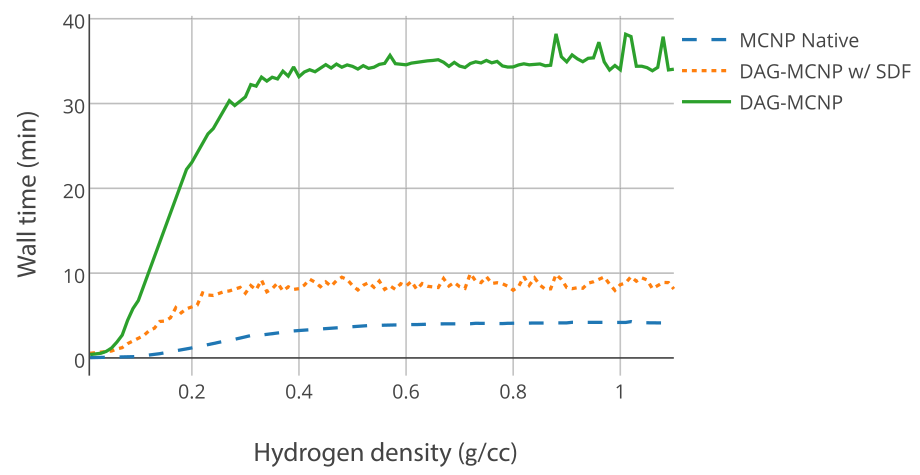
\includegraphics[width=0.48\textwidth]{imgs/sdf-best-case.png}
\caption{\label{fig:sdf-best-case}Performance benefit of \gls{SDF} in an ideal
  case of a 5 MeV neutron point source of neutrons at the center of a 10 cm
  sphere.}
\end{wrapfigure}

A complete implementation of this capability includes tools to assess which
volumes in a geometry will benefit from the initial computational cost and
ongoing memory cost of pre-computing and storing this information.  In
particular, theoretical analysis has shown that the benefit is a function of
the ratio of the mean free path of radiation transport to the mean chord
length within the volume, with maximum benefit arising when this ratio is
low (see Fig.\ \ref{fig:sdf-best-case}).\citeref{shriwise_particle_2017}

Testing has confirmed this behavior in real geometries, with the conclusion
that only some volumes within a geometry benefit from this treatment.  In
fusion energy systems, the most complex volumes are often formed from the
implicit complement, and therefore are considered vacuums.  In such volumes,
the mean free path is infinite, and the utility of this approach offers no
benefit.

Other ongoing improvements began during this period to address other aspects
of the algorithm, including modifications to the way that \glspl{BVH} are
constructed and traversed with the goal of achieving a factor of 2 or more
improvement in computational performance.  \gls{BVH} tree construction
algorithms can be adaptively selected as the tree become deeper to respond to
the particular arrangement of triangles that are the basis for the tree.  In
addition, cpu-level \gls{SIMD} parallelism can be used to traverse the trees
more quickly.\citeref{wald_embree:_2014} Both of these improvements have been
implemented and testing is underway to demonstrate their effectiveness, with
final results expected in summer 2018.

\subsection{\gls{SDR} Workflow Development}

\begin{wrapfigure}{R}{0.5\textwidth}
\centering
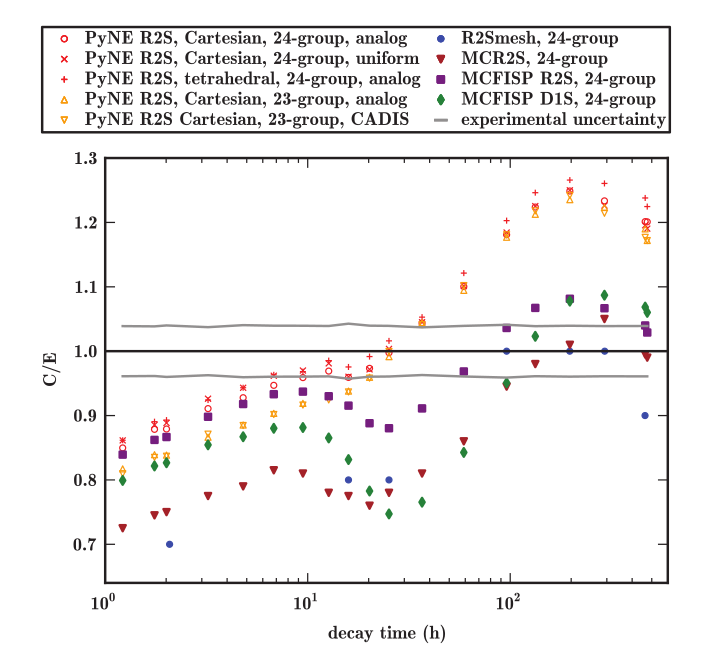
\includegraphics[width=0.48\textwidth]{imgs/r2s-validation.png}
\caption{\label{fig:r2s-validation}Ratio of calculated (C) dose rates to
  experimental (E) dose rates for different configurations of PyNE R2S,
  compared to other reported results.}
\end{wrapfigure}

The objective of this subtask is to provide a robust computational workflow
for predicting the dose rate in a fusion energy system during shutdown
periods, due to neutron activation of components.

With tools readily available to predict nuclear responses to neutron and
photon transport throughout complex fusion energy systems during plasma
operation, much of the fusion neutronics community has turned its attention to
accurately predicting the radiation dose levels caused by delayed photons
during shutdown.  This is important for understanding both the lifetime dose
to some sensitive equipment, as well as the potential dose to workers during
maintenance procedures.  The leading methodology for this kind of analysis is
known as the \gls{R2S} method, because it requires two separate radiation
transport steps, coupled through a transmutation
calculation.\citeref{chen_rigorous_2002,pereslavtsev_novel_2013,davis_benchmarking_2010}
A fully integrated implementation of this workflow was implemented within the
PyNE software system.\citeref{scopatz_pyne_2014,biondo_rigorous_2015}

The \gls{R2S} workflow starts from a single CAD-based \gls{DAGMC} geometry and
a mesh that defines the spatial resolution of the delayed photon source.
These are used to calculate the multi-group neutron flux on that mesh for use
in the activation/transmutation calculation using DAG-MCNP.  The first step of
\gls{R2S} workflow in PyNE uses the geometry and the multi-group neutron
fluxes to automatically write an input file for
ALARA\citeref{wilson_validation_1998} to perform the transmutation calculation.
If the mesh is a non-conformal Cartesian mesh, a \gls{DAGMC}-based ray tracing
method is used to determine the composite material composition in each mesh
voxel for use by ALARA, starting from the same \gls{DAGMC} geometry.  If a
conformal tetrahedral mesh is used, each mesh element is assumed to contain a
single material.

The second step of the \gls{R2S} workflow reads the ALARA output and generates
a spatially distributed multi-group photon source on the same mesh that was
used to record the neutron fluxes.  A different source mesh is generated for
each cooling time, \emph{i.e.} time after shutdown.  A custom source sampling
function is then able to read this mesh-based source, whether Cartesian or
tetrahedral, in the second radiation transport calculation on the original
\gls{DAGMC} geometry.

This particular implementation is innovative in its support for conformal
tetrahedral mesh as well as biasing schemes for efficiently sampling the
distributed photon source, and has been validated against the primary
experimental data for this kind of analysis.\citeref{biondo_shutdown_2016}

Two ongoing improvements that began during this period are an extension to
support moving activated sources during maintenance procedures, and a study of
the propagation of statistical error/uncertainty through the \gls{R2S}
workflow.\citeref{harb_effect_2017}

\subsection{Automated Variance Reduction for \gls{SDR} Analysis}

\begin{wrapfigure}{R}{0.5\textwidth}
\centering
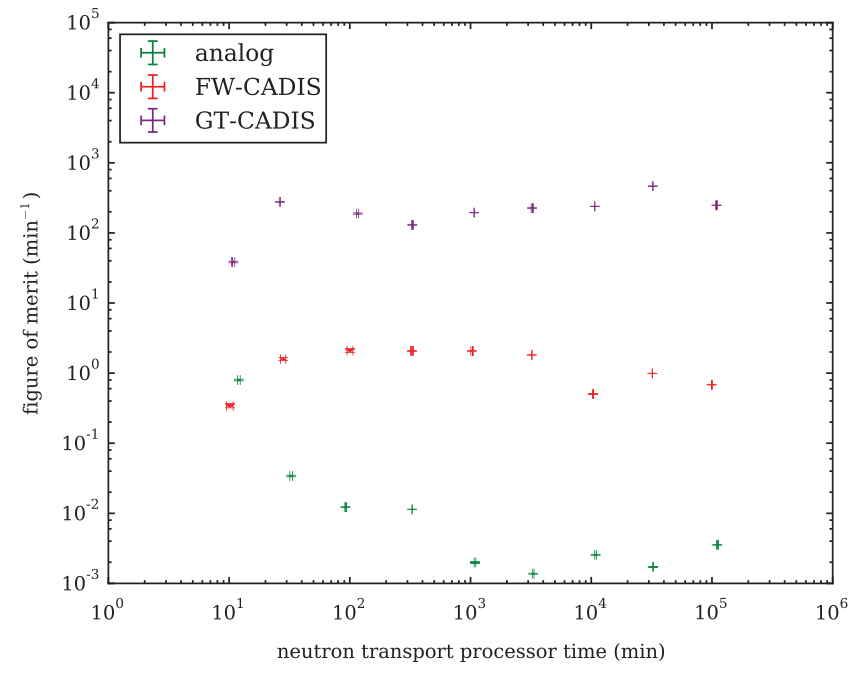
\includegraphics[width=0.48\textwidth]{imgs/gt-cadis-timing.png}
\caption{\label{fig:gt-cadis-timing}Performance benefit of \gls{GT-CADIS}
  compared to \gls{FW-CADIS} and analog simulation.}
\end{wrapfigure}

The objective of this subtask is to develop and demonstrate novel mathematical
approaches that will dramatically increase the statistical convergence rate of
\gls{R2S} simulations.

For over a decade, deterministic radiation transport methods have been used to
determine the variance reduction parameters that allow more accurate Monte
Carlo radiation transport calculations to provide useful answers in a
reasonable computer time.  Although such methods are well-established for the
prompt photons that arise during operational scenarios, the non-linear
relationship between the neutron flux and the delayed photon source of
\gls{R2S} problems has proven challenging.  An extension of the \gls{R2S}
methodology was developed and implemented to overcome this challenge.

The \gls{GT-CADIS} methodology extends the \gls{CADIS} methodology developed
at \gls{ORNL} by implementing a linearization of the transmutation operator
that can be used to couple the adjoint photon flux to the adjoint neutron
source, thus enabling automated variance reduction for \gls{SDR} problems.
The development of this approach required first demonstrating that such a
linearized operator was a sufficiently accurate representation of the
transmutation operator for such problems.  A mathematical derivation
identified the \gls{SNILB} criteria which must be met for this to be correct,
and a thorough analysis of a wide array of fusion materials over many
irradiation conditions confirmed that such criteria are indeed met for all
cases of interest.

The \gls{GT-CADIS} methodology was studied in detail on a simplified geometry
designed to demonstrate the benefit of this approach over other possible
approaches for \gls{SDR} problems.  \gls{GT-CADIS} was found to offer a
substantial speedup over the next best choice, \gls{FW-CADIS}
(Fig.\ \ref{fig:gt-cadis-timing}).\citeref{biondo_transmutation_2017} A single octant model
of a realistic fusion energy system was also used to demonstrate the utility
of this approach.\citeref{biondo_hybrid_2016}

\subsection{Software Validation with JET Operational Data}

The objective of this subtask is to extend the validation basis of \gls{DAGMC}
and the PyNE \gls{R2S} workflow by comparison to additional experimental data.

A collaboration has been established with EURATOM-JET for the neutronics
analysis of JET.  In addition to validating the EU neutronics transport codes
and data, the JET Project, through JET3 - DT Technology EUROfusion Consortium,
would like to widen the scope of JET experiments by also including the
validation of other newly developed transport codes/data used by the US.
Specifically, the collaboration would seek to validate ADVANTG, ATTILA, and
DAG-MCNP, including the \gls{R2S} methodology that relies upon it, by using
the experimental data to be provided by JET.

Two different benchmark exercises were devised, one focusing on streaming of
neutrons and another on the shutdown dose rate.  The former is particularly
valuable for the validation of advanced hybrid variance reduction schemes,
such as ADVANTG.  The other is valuable for validation of \gls{SDR}
calculation methodologies, and particularly the \gls{R2S} methodology
developed under this project.

\begin{wrapfigure}{R}{0.5\textwidth}
\centering
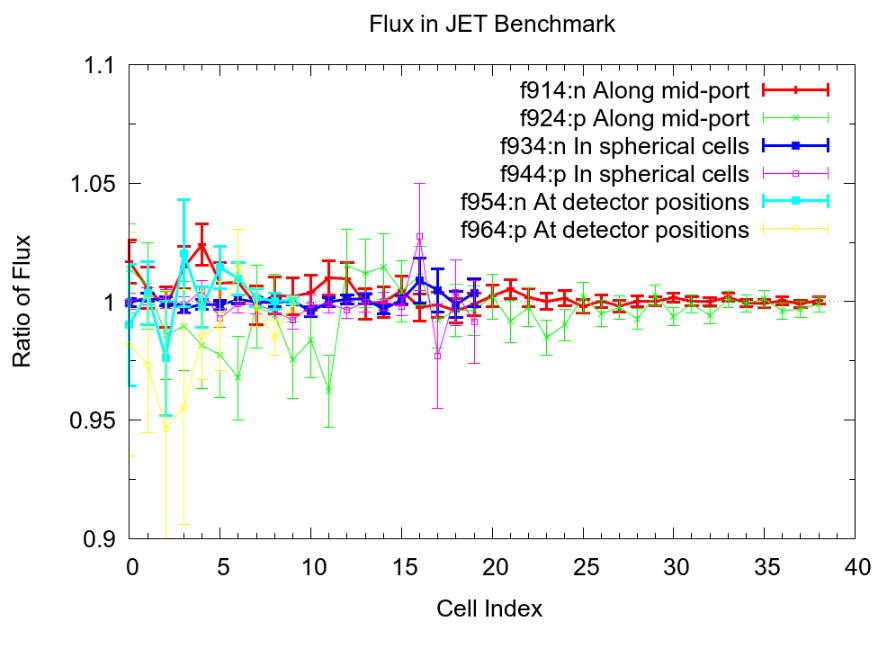
\includegraphics[width=0.48\textwidth]{imgs/jet-streaming-benchmark.png}
\caption{\label{fig:jet-streaming-benchmark}Ratio of DAG-MCNP to MCNP results
  along streaming path in JET model.}
\end{wrapfigure}

Because the geometric description of the JET facility is already available in
the native MCNP text files, participating in this effort required first
generating a \gls{CAD}-based description.  This was performed using the
MCNP2CAD conversion tool developed in conjunction with the \gls{DAGMC}
toolkit.  These \gls{CAD}-based models have already been used to replicate the
streaming benchmark (Fig.\ \ref{fig:jet-streaming-benchmark} and are currently
being used for the \gls{SDR} benchmark.

\subsection{Nuclear Data for Fusion Applications}

The objective of this subtask is to understand the implications of changes in
available best-estimate nuclear data on the analysis and design of fusion
energy systems.

In addition to the tools and workflows described above, robust nuclear
analysis relies on high quality nuclear and atomic data to describe the
interactions of radiation with matter.  Under this project and its
predecessors, we are responsible for monitoring the the development of updated
nuclear data sets and assessing the impacts of those updates on the nuclear
analysis outcomes for various systems.  In addition to attending meetings of
the \gls{CSEWG} and \gls{FENDL} committees, a computational MCNP benchmark is
used to probe the differences in data libraries as they are released.

\begin{wrapfigure}{R}{0.65\textwidth}
\centering
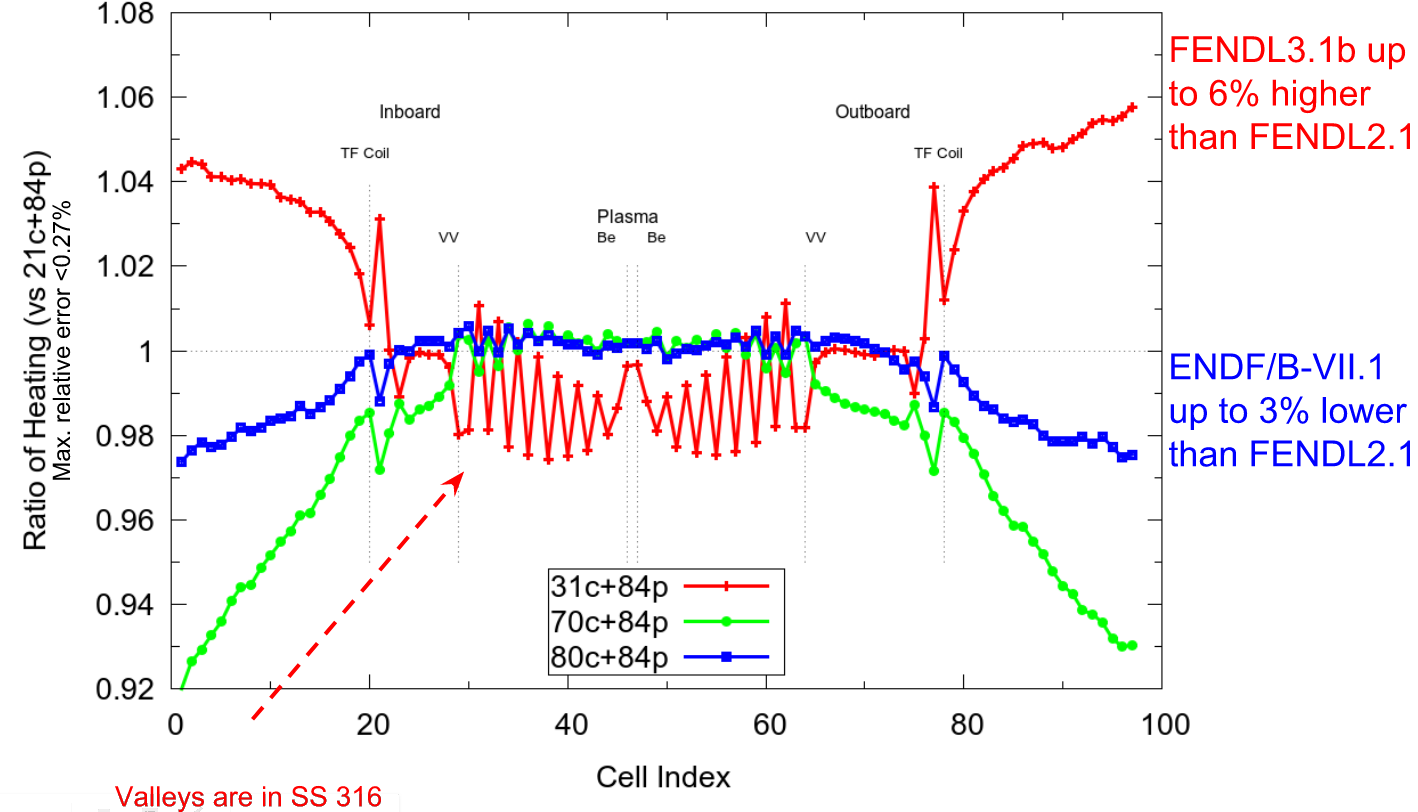
\includegraphics[width=0.63\textwidth]{imgs/fendl3.png}
\caption{\label{fig:fendl3_impact}Impact of FENDL-3.1 library on
  nuclear responses in computational benchmark problem.}
\end{wrapfigure}

During this reporting period, the newest release of the \gls{FENDL}, version
3, was made available.  The computational benchmark was used with the release
of \gls{FENDL}-3, showing a modest increase of the neutron flux levels in the
deep penetration regions and a substantial increase in the gas production in
steel components.  The comparison to experimental results showed good
agreement with no substantial differences between FENDL-3.0 and FENDL-2.1 for
most responses (see Fig.\ \ref{fig:fendl3_impact}).  There is a slight trend,
however, for an increase of the fast neutron flux in the shielding experiment
and a decrease in the breeder mock-up experiments. The photon flux spectra
measured in the bulk shield and the tungsten experiments are significantly
better reproduced with FENDL-3.0 data. In general, FENDL-3, as compared to
FENDL-2.1, shows an improved performance for fusion neutronics
applications. It is thus recommended to ITER to replace FENDL-2.1 as reference
data library for neutronics calculation by
FENDL-3.0.\citeref{fischer_benchmarking_2014, bohm_impact_2015}

In addition to these routine tasks, recent work has also begun investigating
how neutronics results depend on the modeled temperature of various
components.  While most systems are modeled at room temperature, the elevated
temperatures of fusion energy systems during normal operation will impact the
results in three distinct ways: (1) reduced density of materials, (2) Doppler
broadening of nuclear cross-sections, and (3) closing of gaps due to thermal
expansion.  Analysis of these effects shows that the Doppler broadening has a
small impact ($<$1-3\%) on results in fusion energy system, while gap closing
and density reduction can have important effects (4-25\%).

\subsection{Summary}

Overall, this task comprises a comprehensive effort to improve and extend the
available software tools for predictive nuclear analysis of fusion energy
systems.  Novel mathematical and computational approaches are developed to
both improve the performance of existing capability and extend the range of
problems that can be tackled.  Validation is integrated into the development
process using newly available experimental data.

In addition to being used by \gls{UW-FTI} in the Fusion Energy Systems Studies
task described in the next section, this software capability has been used for
analysis of ITER in support of component design and \gls{SDR} throughout the
tokamak building.  In addition to other institutions funded by OFES, a number
of private companies with interest in fusion energy systems have acquired the
software and been trained to use it for a range of analysis tasks.
Internationally, \gls{DAGMC} and related tools have been installed at CCFE,
KIT and ASIPP.  Interest has extended also beyond the fusion neutronics
community, with deployment by and training of nuclear analysis and radiation
transport experts at \gls{SNS}, CEA, CERN and NASA.

